
This section presents the results of an analysis of real-world health data (from the UK Biobank). We are interested in investigating associations between the severity of a COVID-19 infection and various potential risk factors.
This analysis is intended to illustrate the use of the proposed methods in a real-world, mixed variable type example.


\begin{table}[ht]
  \begin{floatrow}
  \ttabbox
  {\caption{Estimated partial correlations between COVID-19 severity and the listed variables for data sets A, B and C.}\label{tab:covid_associations}}
  {\begin{tabular*}{\textwidth}{l @{\extracolsep{\fill}} cccc}
    \\[-1.8ex]\hline 
    \hline \\[-1.8ex]   
    Covid-19 severity assoc. Variables & Data set A & Data set B & Data set C\\
        \hline
        age				 & 0.162  & 0.134   &0.140\\
        waist circ.	     & 0.031  & 0.009	&0.011\\
        deprev. idx      & 0.016  & - 	& -	  \\
        sex				 & 0.007  &	 -      & -	  \\
        hypertension     & 0.075  & 0.035	&0.037\\
        heart attack     &  -     & 0.073   &0.065\\
        diabetes		 & -     & 0.062   &0.055\\
        chr. bronch.     & - &- &   0.012\\
        wisd. teeth surg.& - &  -0.003    & -\\
        \hline
  \end{tabular*}}%
  \end{floatrow}
\end{table}

\subsection{Data set and variables}

We first describe the data set used here, which is a part of the UK Biobank COVID-19 resource in which UK Biobank data were linked to clinical COVID data. To construct an indicator of COVID-19 severity, we consider subjects who tested positive for COVID-19 at some point in 2020. Based on that, we created an indicator variable (COVID severity) to capture whether each subject had a severe outcome within six weeks of infection (meaning either hospitalized, hospitalized, receiving critical care, or died). Around $14\%$ experienced such a severe outcome. \begin{figure}[ht]
    \centering
    %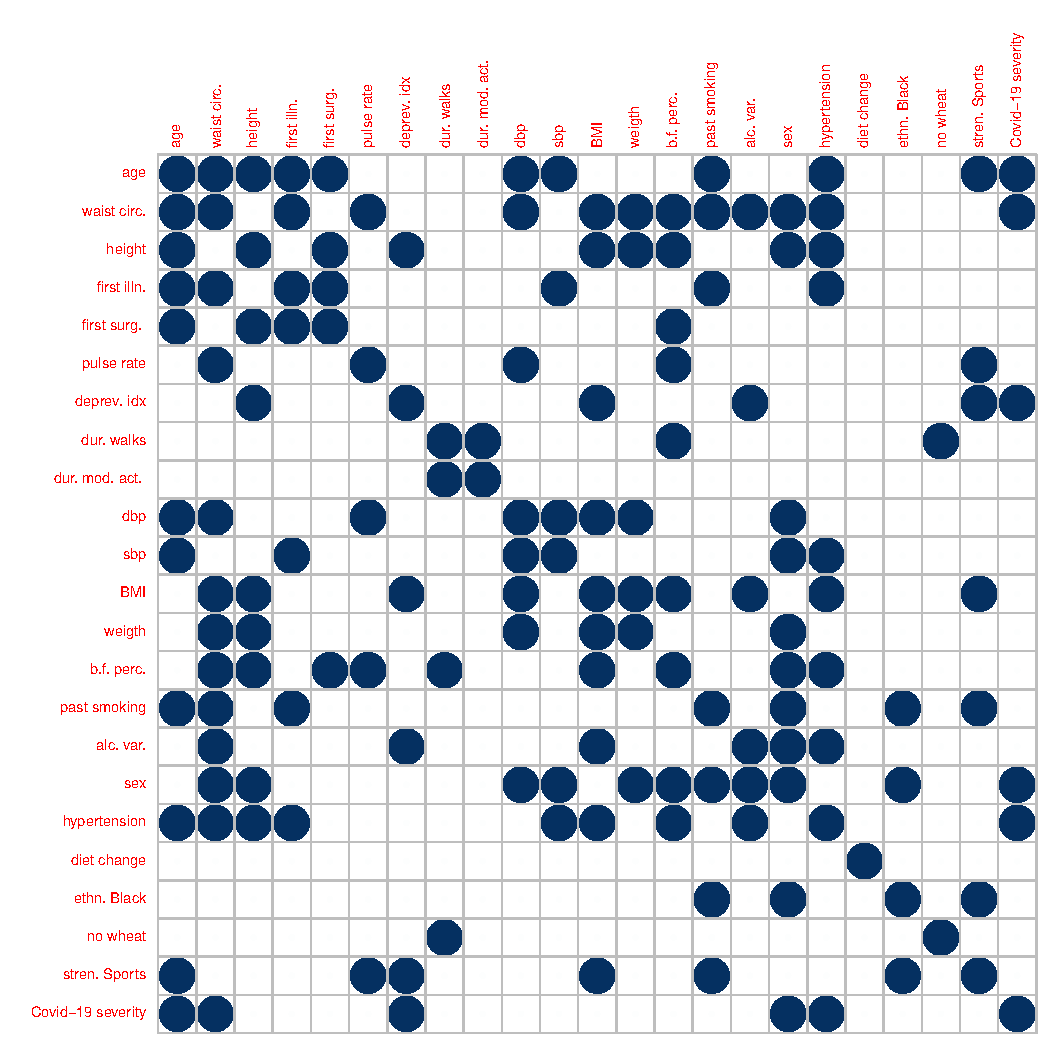
\includegraphics[width=1.00\textwidth]{Figures/corrplot_admat_A.pdf}
    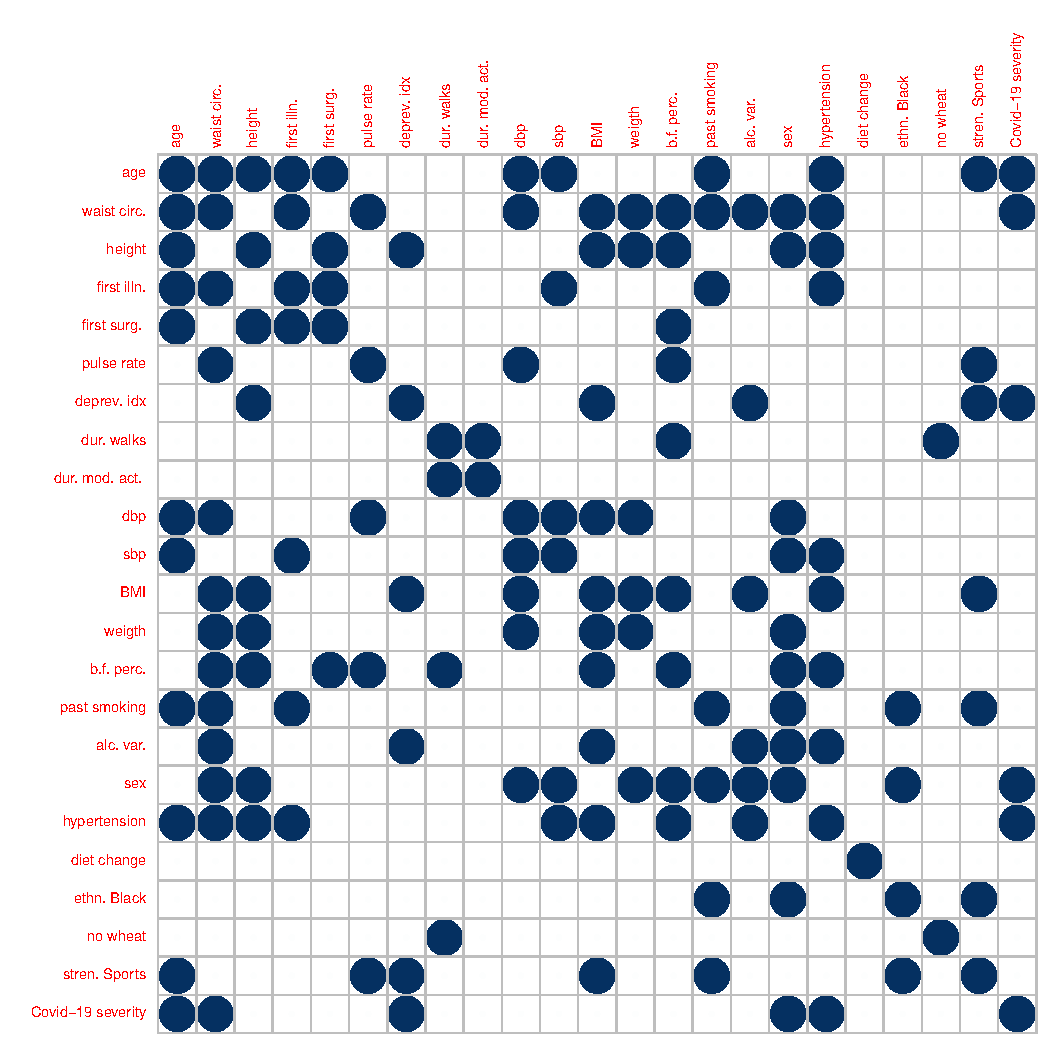
\includegraphics[scale=.6]{Figures/corrplot_admat_A.pdf}
    \caption{Plot of the estimated adjacency matrix of data set A.}
    \label{fig:corrplot_admat_A}
\end{figure}
\begin{figure}[ht]
    \centering
    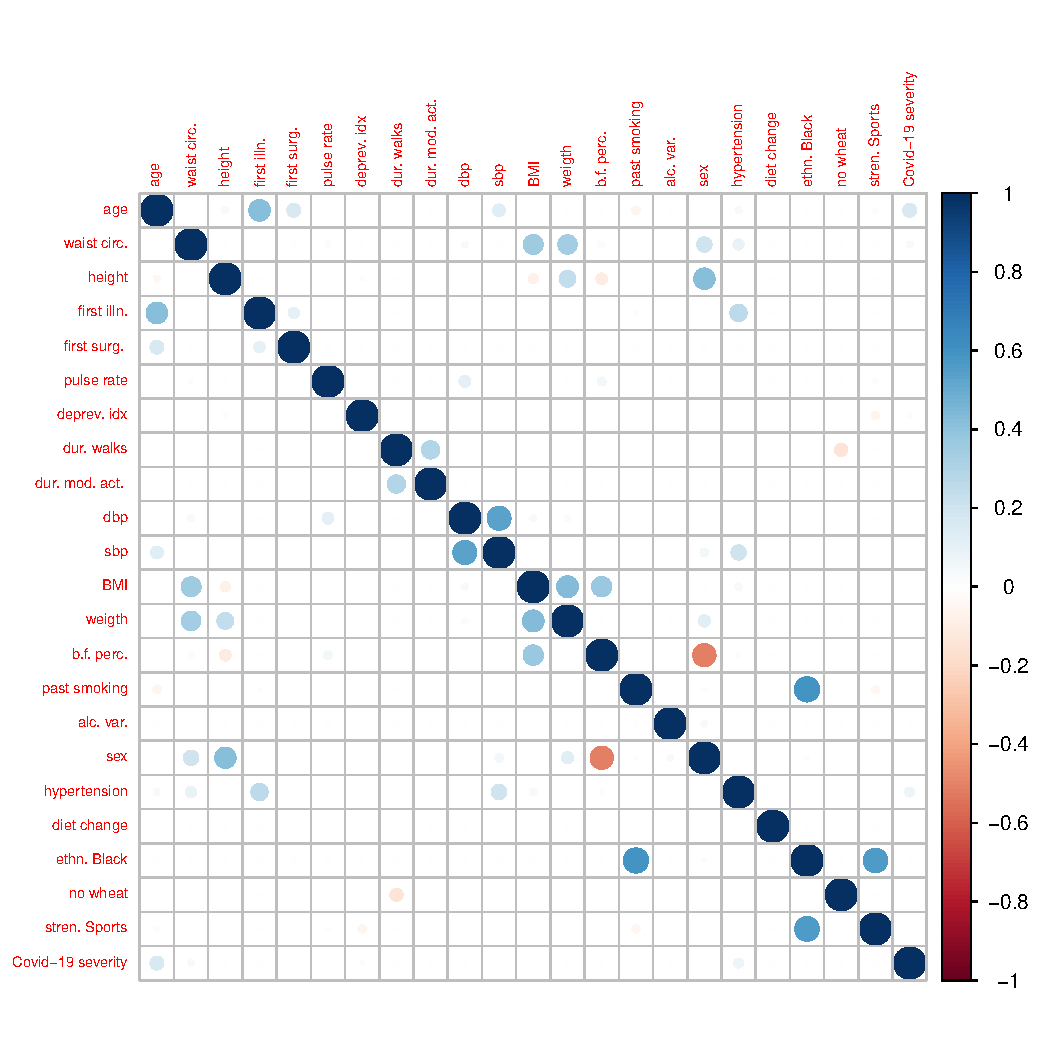
\includegraphics[scale=.6]{Figures/corrplot_omega_A.pdf}
    \caption{Plot of the estimated precision matrix of data set A.}
    \label{fig:corrplot_omega_A}
\end{figure}
The analysis includes $n=8672$ observations on $d=712$ variables (risk factors and covariates with less than 40\% missingness). Missing values were imputed using \texttt{missForest} R-package using default settings. Variables expressing more than $20$ states were treated as continuous. The remaining data include $665$ binary variables, $25$ count variables, and $8$ categorical variables. Many of the binary variables represent the status for relatively rare conditions. This means that the share of the minority class of these indicators (i.e., the fraction of samples with the least frequent value of the variable) can often be minimal. To understand the effects of such rare events on the analysis, we define
three data sets (named A, B, and C) with inclusion rules requiring respectively at least a $25\%, 2\%, 1\%$ share of observations falling into the minority class.

\subsection{Results}

We present the results of a joint analysis of the variables using real UK Biobank data. We emphasize that the analysis aims to illustrate the proposed estimators' behavior and not fully understand the risk factors for severe COVID-19. There has been much work done on factors influencing the risk of severe COVID-19 and its treatment
\citep[see, among others,][]{williamson2020,berlin2020} and we direct the interested reader to the references for further information.

Table \ref{tab:covid_associations} gives a summary of the estimated links (indicated as a visualization of the partial correlations) between the variables (including COVID-19 severity). Considering in particular links to COVID-19 severity, we see that \texttt{age}, \texttt{waist circ.}, \texttt{hypertension}, \texttt{heart attack} and \texttt{diabetes} are quite stable links throughout the different data sets. The effect sizes in terms of partial correlations are penalized and should be interpreted in relative terms. In particular, \texttt{age} retains a relatively large signal, which is in line with the known strong influence of age on COVID-19 severity \citep[see, e.g.][]{williamson2020}.

Finally, we present more detailed results of the analysis of data set A. Figure \ref{fig:corrplot_admat_A} shows the estimated adjacency matrix and Figure \ref{fig:corrplot_omega_A} depicts the estimated precision matrix $\hat{\boldsymbol\Omega}_{A}$. These results highlight the type of output, spanning different kinds of variables, that is readily available from the proposed method.